\documentclass[a4paper,13pt]{report}
\usepackage[table,xcdraw]{xcolor}
\usepackage[normalem]{ulem}
\useunder{\uline}{\ul}{}
\usepackage[utf8]{vietnam}
\usepackage[utf8]{inputenc}
\usepackage{amsmath}
\usepackage{amsfonts}
\usepackage{amssymb}
\usepackage{graphicx}
% \usepackage{caption}
\usepackage{array}
\usepackage{tabularx}
\usepackage[font=small]{caption}
\usepackage{booktabs}
\usepackage[unicode]{hyperref}
\usepackage[left=3cm,right=2cm,top=2.5cm,bottom=3cm]{geometry}
\usepackage{titlesec} 
\usepackage{scrextend}
\usepackage{enumerate}
\usepackage{tikz}
\usepackage{float}
\usepackage{afterpage}
\usepackage{multirow}
\usepackage{sectsty}
\usepackage{tocloft,calc}
\usepackage{listings}
\usepackage{makecell}
% \usepackage[sort&compress]{natbib}
\usetikzlibrary{calc}
\usepackage{algorithm}
% \usepackage[perpage]{footmisc}
\usepackage{perpage} %the perpage package
\MakePerPage{footnote} %the perpage package command
% \usepackage[ruled,vlined]{algorithm2e}
\PassOptionsToPackage{table}{xcolor}

\def\changemargin#1#2{\list{}{\rightmargin#2\leftmargin#1}\item[]}
\let\endchangemargin=\endlist 

\changefontsizes{13pt}
% \bibliographystyle{unsrt}

\makeatletter
\def\l@figure{\@dottedtocline{1}{1em}{2.2em}}
\def\l@table{\@dottedtocline{1}{1em}{2.2em}}
\renewcommand*{\ALG@name}{Thuật toán}
\makeatother

\sectionfont{\fontsize{15}{15}\selectfont}
\subsectionfont{\fontsize{13}{15}\selectfont}

\titleformat{\chapter}[display]   
{\normalfont\huge\bfseries}{\chaptertitlename\ \thechapter}{0pt}{\LARGE}
\titlespacing*{\chapter}{0cm}{-\topskip}{0pt}[0pt]

\renewcommand{\baselinestretch}{1.3}
%\renewcommand{\cftsecpresnum}{Chương\space}
\renewcommand{\cftchappresnum}{Chương }
\AtBeginDocument{\addtolength\cftchapnumwidth{\widthof{\bfseries Chương }}}
\setlength{\parskip}{0.4em}
\setlength{\parindent}{0pt}
%
\title{Một số phương pháp phân loại thực khuẩn}	%% title
\author{Trịnh Bá Tú, Vũ Quang Sơn, Lê Thế Nam}			%% author's name

%
\newcommand{\argmax}{\arg\!\max}

\begin{document}
% Cover Vietnamese 1

% Cover Vietnamese 1

% Cover english
\pagenumbering{gobble}
\begin{center}
	
\begin{tikzpicture}[overlay,remember picture]
	    \draw [line width=3pt,rounded corners=0pt,
	        ]
	        ($ (current page.north west) + (25mm,-25mm) $)
	        rectangle
	        ($ (current page.south east) + (-15mm,25mm) $);
	    \draw [line width=1pt,rounded corners=0pt]
	        ($ (current page.north west) + (26.5mm,-26.5mm) $)
	        rectangle
	        ($ (current page.south east) + (-16.5mm,26.5mm) $);
	\end{tikzpicture}
	\\[1mm]
	%%12pt
	\textbf{ĐẠI HỌC QUỐC GIA HÀ NỘI\\TRƯỜNG ĐẠI HỌC CÔNG NGHỆ}\\[1cm]
	
\includegraphics[width=0.2\linewidth]{figures/uet}\\[0.3cm]
	% \textbf{Ngô Kiên Tuấn}
	% \\[2cm]
	
	\large{\textbf{TỔNG QUAN VỀ PHƯƠNG PHÁP PHÂN LOẠI THỰC KHUẨN DỰA TRÊN TÍNH TOÁN}}
	\\[2.6cm]
	\normalsize{\textbf{BÁO CÁO MÔN HỌC
		\\[2mm]
	INT 7021 - Tin sinh học cho dữ liệu lớn}}

	\vfill
	\textbf{HÀ NỘI - 2025}
	\vspace{10mm}
\end{center}

\begin{center}
	
	
\begin{tikzpicture}[overlay,remember picture]
	\draw [line width=3pt,rounded corners=0pt,
	]
	($ (current page.north west) + (25mm,-25mm) $)
	rectangle
	($ (current page.south east) + (-15mm,25mm) $);
	\draw [line width=1pt,rounded corners=0pt]
	($ (current page.north west) + (26.5mm,-26.5mm) $)
	rectangle
	($ (current page.south east) + (-16.5mm,26.5mm) $);
	\end{tikzpicture}
	\\[1mm]
	\textbf{ĐẠI HỌC QUỐC GIA HÀ NỘI\\TRƯỜNG ĐẠI HỌC CÔNG NGHỆ}
	\\[1cm]
	
\includegraphics[width=0.2\linewidth]{figures/uet}
	\\[0.3cm]
	% \textbf{Ngô Kiên Tuấn}
	% \\[2cm]
	
	\large{\textbf{TỔNG QUAN VỀ PHƯƠNG PHÁP PHÂN LOẠI THỰC KHUẨN DỰA TRÊN TÍNH TOÁN}}
	\\[2.6cm]
	\normalsize{\textbf{BÁO CÁO MÔN HỌC
		\\[2mm]
	INT 7021 - Tin sinh học cho dữ liệu lớn}}
\end{center}
\vspace{16mm}
\begin{center}
\begin{tabular}{r l}
\textbf{Cán bộ hướng dẫn:} & \textbf{TS. Hoàng Thị Điệp} \\
& \textbf{TS. Đặng Cao Cường} \\
& \\
\textbf{Nhóm học viên:} & \textbf{23025097 - Trịnh Bá Tú} \\
& \textbf{23025086 - Vũ Quang Sơn} \\
& \textbf{23025079 - Lê Thế Nam} \\
\end{tabular}
\end{center}

\vfill
\begin{center}
	\textbf{HÀ NỘI - 2025}
	\vspace{10mm}
\end{center}


\newpage\cleardoublepage

% Acknowledgement
% \input{chapters/acknowledgement}\newpage\cleardoublepage
% Assurance
% \input{chapters/assurance}\newpage\cleardoublepage
% Abstract Vietnamese

% Abstract English
% \input{chapters/abtract_en}\newpage\cleardoublepage
\addcontentsline{toc}{chapter}{Mục lục}
\tableofcontents\newpage\cleardoublepage
%

\newpage
\addcontentsline{toc}{chapter}{\listfigurename}
\listoffigures\cleardoublepage

\newpage
\addcontentsline{toc}{chapter}{\listtablename}
\listoftables

\newpage
\chapter*{Danh mục các từ viết tắt}
\addcontentsline{toc}{chapter}{Danh mục các từ viết tắt}
 
%\begin{tabular}{|l|l|l|l|}
\begin{tabular}{|m{1cm}|m{3cm}|m{4cm}|m{6cm}|}
    \hline
\textbf{STT} & \textbf{Từ viết tắt} & \textbf{Cụm từ đầy đủ (tiếng Anh)} & \textbf{Giải nghĩa tiếng Việt} \\
\hline
1 & Phage & Bacteriophage & Thực khuẩn - virus ký sinh trên vi khuẩn \\
\hline
2 & Virulent phage & Virulent phage & Thực khuẩn thể độc lực \\
\hline
3 & Temperate phage & Temperate phage & Thực khuẩn thể ôn hòa \\
\hline
4 & Lytic cycle & Lytic cycle & Chu kỳ tan \\
\hline
5 & Lysogenic cycle & Lysogenic cycle & Chu kỳ tiền tan \\
\hline
6 & Genome & Genome & Bộ gen \\
\hline
7 & Contig & Contig & Đoạn trình tự liên tiếp \\
\hline
8 & NGS & Next-Generation Sequencing & Giải trình tự thế hệ tiếp theo \\
\hline
9 & k-mer & k-mer & Đoạn con độ dài k \\
\hline
10 & Sliding window & Sliding window & Cửa sổ trượt – kỹ thuật cắt chuỗi \\
\hline
11 & AUC & Area Under Curve & Diện tích dưới đường cong ROC \\
\hline
12 & MetaSim & MetaSim & Trình mô phỏng dữ liệu giải trình tự \\
\hline
\end{tabular}
\newpage\cleardoublepage
%\listoftables
\begin{center}
\textbf{\large{Tóm tắt}	}
\end{center}

\addcontentsline{toc}{chapter}{Tóm tắt}

\begin{small}
Thực khuẩn là các vi-rút có khả năng xâm nhiễm vào vi khuẩn. Dựa trên chu kỳ sống, thực khuẩn được phân thành hai nhóm chính. Nhóm thứ nhất là thực khuẩn thể độc lực, thực hiện chu kỳ tan, trong đó thực khuẩn nhân lên nhanh chóng và phá hủy tế bào vi khuẩn sau khi xâm nhiễm. Nhóm thứ hai là thực khuẩn thể ôn hòa, có khả năng tích hợp bộ gen của mình vào nhiễm sắc thể của vi khuẩn và sao chép cùng tế bào chủ thông qua chu kỳ tiềm tan. Từ đó, việc xác định chính xác chu kỳ sống của thực khuẩn là một bước quan trọng trong việc phát triển các ứng dụng phù hợp, đặc biệt trong trị liệu bằng phage, một lựa chọn tiềm năng cho các bệnh nhân dị ứng hoặc kháng thuốc kháng sinh.

Trước đây, các phương pháp phân loại thực khuẩn truyền thống chủ yếu dựa trên nuôi cấy trong phòng thí nghiệm, vốn đòi hỏi nhiều thời gian, chi phí cao và không hiệu quả khi xử lý khối lượng lớn dữ liệu chưa được gán nhãn. Hiện nay, dữ liệu di truyền ngày càng phong phú, được thu thập từ các nguồn như NCBI, PhageScope hay PhageDB cho phép thực hiện các phương pháp phân loại phage dựa trên tính toán. Với sự phát triển của công nghệ, các kỹ thuật học máy và học sâu đã được áp dụng để thực hiện phân loại thực khuẩn đạt được các kết quả tốt và rút ngắn thời gian phân loại so với các phương pháp truyền thống.

Mục tiêu của báo cáo là cung cấp một cái nhìn tổng quan và hệ thống về bài toán phân loại thực khuẩn dựa trên phương pháp tính toán. Trong báo cáo này, nhóm sinh viên chia các phương pháp thành hai nhóm chính: (1) các phương pháp học máy truyền thống giải quyết bài toán với dữ liệu bộ gen đầy đủ (PHACTS, PhageAI, BACPHLIP), và (2) các phương pháp học sâu có khả năng xử lý bài toán với dữ liệu không hoàn chỉnh (DeePhage, PhaTYP, DeepPL).

Báo cáo gồm có 4 chương:
\begin{enumerate}
    \item \textbf{Giới thiệu.} Nội dung của chương này là giới thiệu về các khái niệm liên quan, phát biểu bài toán và nguồn dữ liệu.
    \item \textbf{Các nghiên cứu liên quan.} Chương này tập trung trình bày về các phương pháp phân loại thực khuẩn dựa trên tính toán tiêu biểu.
    \item \textbf{Thực nghiệm.} Chương này trình bày về dữ liệu, kịch bản, chỉ số, kết quả liên quan tới các thực nghiệm mà nhóm sinh viên đạt được.
    \item \textbf{Kết luận.} Trong chương này, nhóm sinh viên tập trung thảo luận về kết quả đạt được và hướng nghiên cứu tiếp theo.
\end{enumerate}
% \vspace*{1cm}
% \textbf{Từ khóa}: \textit{hệ thống dòng sản phẩm}, \textit{kiểm thử phần mềm}, \textit{sinh ca kiểm thử}, \textit{kiểm thử đột biến}, \textit{dữ liệu đánh giá}

\end{small}\newpage\cleardoublepage

%
\chapter{Mở đầu}
% \addcontentsline{toc}{chapter}{Mở đầu}
\setcounter{page}{1}
\pagenumbering{arabic}
\section{Giới thiệu}

\subsection{Vi khuẩn, vi-rút và thực khuẩn}

Vi khuẩn là sinh vật đơn bào có kích thước nhỏ (0,2 - 5 µm), có cấu tạo đơn giản bao gồm tế bào chất, màng tế bào và vách tế bào. Vi khuẩn sinh sản chủ yếu bằng phương pháp phân đôi. Ngược lại, vi-rút không phải là sinh vật sống hoàn chỉnh do không có cấu trúc tế bào, mà chỉ bao gồm vật liệu di truyền (ADN hoặc ARN) được bao bọc bởi lớp vỏ protein. Vi-rút chỉ có thể sao chép khi xâm nhập vào tế bào vật chủ và khai thác bộ máy sinh học của tế bào đó.

Trong nhóm vi-rút, \textbf{thực khuẩn} là loại xâm nhiễm vào vi khuẩn. Mỗi loại vi khuẩn thường bị nhiễm bởi một hoặc một vài loại thực khuẩn đặc trưng. Thực khuẩn đóng vai trò quan trọng trong điều hòa quần thể vi khuẩn tự nhiên và đang được nghiên cứu ứng dụng trong y học. Dựa trên chu kì sống bên trong vi khuẩn, thực khuẩn được chia thành hai nhóm chính: \textbf{Thực khuẩn thể độc lực} và \textbf{thực khuẩn thể ôn hoà}. Với thực khuẩn thể độc lực, sau khi xâm nhập vào tế bào vi khuẩn, thực khuẩn chiếm quyền kiểm soát, nhân bản, và phá hủy tế bào để giải phóng các bản sao mới, quá trình này được gọi là \textbf{chu kỳ tan}. Với thực khuẩn thể ôn hoà, chúng tích hợp vật liệu di truyền của mình vào hệ gen của vi khuẩn, nhân bản cùng vật chủ mà không phá hủy tế bào, quá trình này gọi là \textbf{chu kỳ tiền tan} và có thể chuyển sang chu kỳ tan khi gặp điều kiện kích hoạt.


\subsection{Động lực thúc đẩy}

Việc phân loại thực khuẩn là có độc lực hay ôn hòa mang đến những lợi ích to lớn cho việc nghiên cứu hệ vi sinh vật và ứng dụng của chúng. Đầu tiên, phân loại thực khuẩn là chìa khóa để khám phá mối quan hệ phức tạp giữa thực khuẩn và vật chủ, từ đó làm sáng tỏ vai trò của thực khuẩn trong cộng đồng vi sinh vật. Tiếp theo, việc nhận diện chính xác thực khuẩn có độc lực là bước đệm quan trọng cho việc phát triển các liệu pháp điều trị bằng thực khuẩn, nhằm tiêu diệt các vi khuẩn gây bệnh, mở ra hướng đi mới cho việc điều trị.
Để phân loại một thực khuẩn mới có thuộc loại nào, chúng cần được nuôi cấy trong phòng thí nghiệm và theo dõi. Các kỹ thuật nuôi cấy này không chỉ tốn thời gian và chi phí mà còn không có khả năng áp dụng được đối với các trình tự thực khuẩn mới được tổng hợp từ môi trường. Do đó, một phương pháp phân loại thực khuẩn dựa trên tính toán thông qua dữ liệu trình tự gen của thực khuẩn là cần thiết.

Với mục tiêu cải tiến phương pháp cũ hay phát triển phương pháp mới, báo cáo này cung cấp một góc nhìn tổng quan về các phương pháp tiêu biểu đã được công bố, giúp tiếp cận bài toán phân loại thực khuẩn dựa trên tính toán một cách khái quát và nhanh chóng nhất.

\section{Phát biểu bài toán}

Trong bối cảnh số lượng lớn thực khuẩn được phát hiện thông qua các công nghệ giải trình tự thế hệ mới, việc phân loại thực khuẩn bằng các phương pháp truyền thống là rất tốn kém, về cả nguồn lực và tài chính. Cùng với sự phát triển của công nghệ tính toán, các phương pháp học máy và học sâu được sử dụng để thực hiện phân loại thực khuẩn.

\subsection{Định nghĩa bài toán}
\begin{figure}[H]
    \centering
    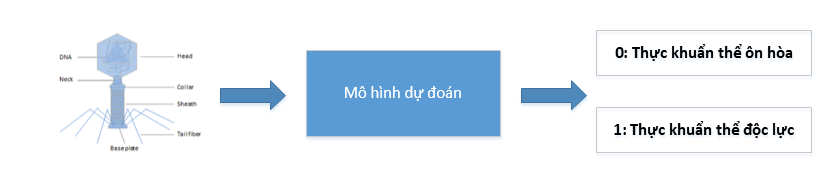
\includegraphics[width=1\linewidth]{figures/problem.png}
    \caption{Sơ đồ mô tả bài toán phân loại thực khuẩn dựa trên tính toán}
    \label{fig:problem}
\end{figure}

Hình \ref{fig:problem} mô tả bài toán phân loại thực khuẩn dựa trên phương pháp tính toán, trong đó:
\begin{itemize}
    \item \textbf{Dữ liệu đầu vào}: Chuỗi DNA đầy đủ hoặc tập hợp các đoạn DNA ngắn được lấy từ bộ gen của thực khuẩn.
    \item \textbf{Mô hình dự đoán}: Thuật toán học máy, học sâu được huấn luyện.
    \item \textbf{Dữ liệu đầu ra}: Dự đoán thực khuẩn là thể có độc lực hay thể ôn hòa.
\end{itemize}

\subsection{Đặc điểm của bài toán}

\begin{itemize}
    \item Xét ở khía cạnh học máy, bài toán phân loại thực khuẩn là bài toán phân loại nhị phân (\textit{binary classification}).
    \item Dữ liệu đầu vào có độ dài và chất lượng không đồng đều, bao gồm cả các trình tự ngắn hoặc có chứa nhiễu sinh học.
    \item Các mô hình cần đảm bảo tính chính xác cao, khả năng khái quát tốt với dữ liệu chưa thấy trong quá trình huấn luyện.
    \item Phải xử lý được dữ liệu có nguồn gốc từ các họ thực khuẩn khác nhau và có tính đa dạng về mặt di truyền học.
\end{itemize}

\subsection{Thách thức trong quá trình thực hiện}
Với cách tiếp cận dựa trên tính toán, việc phân loại thực khuẩn hiện tại đang gặp phải 4 khó khăn chính:
\begin{enumerate}
    \item \textbf{Thiếu dữ liệu huấn luyện chất lượng cao}: Mặc dù số lượng thực khuẩn trong tự nhiên được ước tính lên đến khoảng $10^{31}$ \cite{doi:10.1128/jb.00052-20}, nhưng hiện nay chỉ có một lượng rất nhỏ bộ gen thực khuẩn đã được giải trình tự hoàn chỉnh và đưa vào cơ sở dữ liệu. Phần lớn các thực khuẩn này vẫn chưa được xác định đặc điểm sinh học cụ thể, bao gồm cả thông tin về vòng đời (chu kỳ sinh tan hay tiềm tan). Điều này dẫn đến sự thiếu hụt dữ liệu được gán nhãn rõ ràng và chính xác, gây khó khăn cho quá trình huấn luyện các mô hình học máy trong bài toán phân loại vòng đời thực khuẩn.
    \item \textbf{Không tồn tại chỉ dấu sinh học phổ quát}: Không giống như vi khuẩn có gen 16S rRNA được bảo tồn cao, đóng vai trò như một chỉ dấu phân tử phổ quát trong phân loại và phân tích phát sinh loài, thực khuẩn không sở hữu bất kỳ gen nào có mặt đồng nhất và bảo tồn trên toàn bộ các nhóm thực khuẩn \cite{PMID:31061483}. Do đó, việc phân loại thực khuẩn thường dựa trên nội dung bộ gen hoặc các gen đặc trưng cho từng nhóm nhỏ.
    \item \textbf{Tính tương đồng di truyền với vật chủ}: Nhiều đoạn gen của phage có thể có trình tự tương tự hoặc thậm chí đồng nhất với gen vi khuẩn, do quá trình tiến hóa đồng hành hoặc sự trao đổi gen thông qua cơ chế di truyền ngang.
    \item \textbf{Xử lý dữ liệu không đầy đủ}: Trong những nghiên cứu gần đây, dữ liệu được thu thập thông qua metagenomics – phương pháp giải trình tự toàn bộ DNA có trong mẫu môi trường (như đất, nước, ruột sinh vật) mà không cần phải nuôi cấy vi sinh vật trong phòng thí nghiệm. Tuy nhiên, một đặc điểm hạn chế của phương pháp này là chỉ thu được các đoạn DNA ngắn, rời rạc và không hoàn chỉnh, thay vì toàn bộ bộ gen đầy đủ của một loại thực khuẩn. Điều này gây khó khăn vì các đoạn trình tự thu được có thể không chứa đủ thông tin đặc trưng, dễ bị nhiễu hoặc nhầm lẫn với vật liệu di truyền từ các sinh vật khác trong mẫu. Do đó, việc xử lý dữ liệu từ metagenomics đòi hỏi các phương pháp phân tích chuyên biệt để bù đắp cho tính không đầy đủ và phân mảnh của dữ liệu..
\end{enumerate}

Với các đặc điểm nêu trên, bài toán phân loại thực khuẩn đòi hỏi sự kết hợp giữa kiến thức sinh học phân tử và các kỹ thuật trong lĩnh vực học máy và học sâu. Đây chính là trọng tâm của các phương pháp được khảo sát trong báo cáo này.

\section{Nguồn dữ liệu và định dạng dữ liệu}

\subsection{Nguồn dữ liệu}

Các phương pháp phân loại được đề cập đến trong báo cáo này lấy dữ liệu từ các nguồn sau:

\begin{itemize}
    \item \textbf{NCBI (National Center for Biotechnology Information - \url{https://www.ncbi.nlm.nih.gov/})}: Là một trong những kho dữ liệu sinh học lớn và toàn diện nhất, chứa thông tin về trình tự DNA, protein, gen, và các chú thích liên quan. NCBI cung cấp cả dữ liệu thô và đã được gán nhãn, là nguồn phổ biến cho việc huấn luyện và đánh giá mô hình phân loại.
    
    \item \textbf{PhageScope - \url{https://phagescope.deepomics.org/database}}: Là cơ sở dữ liệu chuyên biệt dành cho thực khuẩn, hỗ trợ phân tích chức năng, xác định vòng đời và các đặc điểm phân tử. PhageScope tích hợp các công cụ tính toán, hỗ trợ xử lý và khám phá dữ liệu thực khuẩn ở mức độ chi tiết.
    
    \item \textbf{PhageDB - \url{https://phagesdb.org}}: Là kho dữ liệu tập trung vào thu thập và lưu trữ thông tin thực nghiệm về các chủng thực khuẩn đã được phát hiện. PhageDB thường được sử dụng để đánh giá mô hình phân loại trên các bộ dữ liệu thực tế.
\end{itemize}

\subsection{Định dạng dữ liệu}

Khi xử lý dữ liệu thực khuẩn, hai định dạng tập tin phổ biến là \texttt{FASTA} và \texttt{GenBank}. Mỗi định dạng cung cấp một cách biểu diễn riêng cho trình tự nucleotide và thông tin liên quan.

\subsubsection{Định dạng FASTA}

Định dạng \texttt{FASTA} là định dạng văn bản đơn giản dùng để lưu trữ trình tự nucleotide hoặc amino acid. Tệp tin định dạng FASTA có phần mở rộng là *.fasta. Cấu trúc của tập tin FASTA bao gồm hai phần:

\begin{itemize}
    \item \textbf{Dòng tiêu đề} (header): Bắt đầu bằng ký tự \texttt{>}, tiếp theo là thông tin mô tả, thường bao gồm ID chuỗi, tên sinh vật, tên gen hoặc nguồn gốc.
    \item \textbf{Trình tự} (sequence): Nằm ở các dòng tiếp theo, chứa các ký tự đại diện cho nucleotide (\texttt{A}, \texttt{T}, \texttt{G}, \texttt{C}) hoặc acid amin.
\end{itemize}

\noindent Ví dụ: file $NC\_000866\_Lytic.fasta$ có nội dung như sau:
\begin{verbatim}
>NC_000866.4 Enterobacteria phage T4, complete genome
AATTTTCCTTATTAGGCCGCAAGGGCCTTCATAGTTTTAGCGATTTGGGAAACTTCATCA
TCACTTAAAGAGTTGCGATAACCGATGAAGTCGGAAACAATACGGAATTTCTTGGTAAAC
TCAGCAACCATTTTATCACTGTTTTTTGAAGCATTATTTGATAATACATCAAAAAGATTA
GTTACTGTCCAAATGTCATGACCGATGGTATCTTTTCCACCATTAAAATATACACCCTGT
.....
\end{verbatim}

\subsubsection{Định dạng GenBank}

Định dạng \texttt{GenBank} là định dạng tiêu chuẩn của NCBI, chứa thông tin chi tiết hơn so với FASTA. Tệp tin định dạng FASTA có phần mở rộng là *.gb.  Một tệp tin GenBank bao gồm ba phần chính:

\begin{itemize}
    \item \textbf{Phần tiêu đề} (Header): Mô tả chung về bộ gen, bao gồm số hiệu truy cập, nguồn sinh vật, độ dài chuỗi và các đặc điểm chung.
    \item \textbf{Phần đặc trưng} (Features): Liệt kê các đặc trưng sinh học của chuỗi, bao gồm vị trí gen, loại protein mã hóa, chú thích chức năng.
    \item \textbf{Phần trình tự} (Sequence): Trình bày toàn bộ chuỗi nucleotide của bộ gen.
\end{itemize}

Ví dụ dưới đây là một phần của file $AF503408\_Lysogneic.gb$
\begin{verbatim}
LOCUS       AF503408    101660 bp    DNA     linear   PHG 28-APR-2006
DEFINITION  Enterobacteria phage P7, complete genome.
ACCESSION   AF503408
.....
FEATURES             Location/Qualifiers
     source          1..101660
                     /organism="Enterobacteria phage P7"
                     /mol_type="genomic DNA"
                     /db_xref="taxon:10682"
....
ORIGIN      
  1 acattatacg aagttatatt aagggttatt gaacatgatc aatttacctg taaatccata
 61 cagttcaata ccttatcagg tcaaatagtg atcacttgat catttgatca agtttgcgct
121 acgtaaaatc tgtgaaaagt tggcagtgtt agtgctccag atttcgcgta gcgcacttag
181 caccaccaat caatcagagg tgaaaaatgg gatattcagc tgctaaagtg tccactcatc
241 ttgagcttga gaaaaaccgt ggttactggc gggcaaaagg gtttgatcgt gatagttgcc
301 aactgtcatt atcgcgcggt gaagagaaaa tagtacgcac gcgcggtcgc tggcgtttct
\end{verbatim}


Định dạng GenBank hỗ trợ các phần mềm sinh học phân tử và hệ thống phân tích chú thích gen trong quá trình tiền xử lý dữ liệu.

\cleardoublepage\newpage\cleardoublepage
\chapter{Các nghiên cứu liên quan}

Chương này trình bày tổng quan và phân tích các phương pháp phân loại thực khuẩn dựa trên dữ liệu di truyền. Hai tiêu chí chính được sử dụng để tổ chức và đánh giá các phương pháp bao gồm: (1) phân loại theo loại thuật toán học máy được áp dụng, và (2) sắp xếp theo trình tự thời gian công bố nhằm phản ánh tiến trình phát triển của lĩnh vực.

\section{Phân loại theo phương pháp học máy}

Dựa trên kỹ thuật xử lý dữ liệu và loại mô hình học máy sử dụng, các phương pháp phân loại thực khuẩn có thể chia thành hai nhóm chính:

\begin{itemize}
    \item \textbf{Nhóm 1:} Các phương pháp học máy truyền thống, sử dụng các thuật toán như Random Forest (Rừng ngẫu nhiên), SVM (Support Vector Machine - Máy vector hỗ trợ), v.v. với đầu vào là bộ gen thực khuẩn đầy đủ. Báo cáo này thực hiện trên 3 phương pháp của \textbf{PHACTS}, \textbf{PhageAI}, và \textbf{BACPHLIP}.
    
    \item \textbf{Nhóm 2:} Các phương pháp học sâu, có khả năng xử lý dữ liệu không hoàn chỉnh nên có khả năng tận dụng được lượng dữ liệu lớn từ nguồn dữ liệu metagenomics. Báo cáo này thực hiện trên 3 phương pháp của \textbf{DeePhage}, \textbf{PhaTYP}, và \textbf{DeepPL}.
\end{itemize}

\section{Sắp xếp theo thứ tự thời gian công bố}

Bên cạnh phân loại theo kỹ thuật, các phương pháp còn được trình bày theo thứ tự thời gian công bố để thể hiện xu hướng phát triển qua các giai đoạn và so sánh kết quả của phương pháp mới với phương pháp trước đó. Thời gian công bố của từng phương pháp như sau:

\begin{enumerate}
    \item \textbf{PHACTS} – tháng 01 năm 2012
    \item \textbf{PhageAI} – tháng 07 năm 2020
    \item \textbf{BACPHLIP} – tháng 05 năm 2021
    \item \textbf{DeePhage} – tháng 09 năm 2021
    \item \textbf{PhaTYP} – tháng 01 năm 2023
    \item \textbf{DeepPL} – tháng 10 năm 2024
\end{enumerate}

\section{Phương pháp trình bày trong các phần tiếp theo}

Để đảm bảo tính nhất quán và thuận tiện cho việc đánh giá, mỗi phương pháp được trình bày một số điểm chính bao gồm:

\begin{enumerate}
    \item \textbf{Mô tả chung} về phương pháp, động lực, phương pháp thực hiện và mục tiêu.
    \item \textbf{Tập dữ liệu:} Mô tả nguồn dữ liệu, số lượng mẫu, tính chất dữ liệu (hoàn chỉnh hay contig), và phương pháp gán nhãn.
    \item \textbf{Phương pháp thực hiện:} Thuật toán hoặc mô hình được áp dụng, kiến trúc mạng (nếu có), kỹ thuật xử lý đặc trưng và quy trình huấn luyện.
    \item \textbf{Kết quả thu được:} Các chỉ số đánh giá như độ chính xác, độ nhạy, độ đặc hiệu, F1-score, v.v..
    \item \textbf{So sánh với các phương pháp trước:} Ưu điểm nổi bật, cải tiến kỹ thuật, sự khác biệt về khả năng dự đoán.
\end{enumerate}
\newpage\cleardoublepage
\section{PHACTS}

PHACTS\cite{mcnair2012phacts} là một trong những công cụ tiên phong trong việc phân loại thực khuẩn thể theo vòng đời dựa trên bộ gen đầy đủ. Công cụ này sử dụng thuật toán \textbf{Random Forest (Rừng ngẫu nhiên)} để xây dựng mô hình học máy dựa trên mức độ tương đồng protein giữa các thực khuẩn.

\subsection{Dữ liệu huấn luyện}

\begin{itemize}
    \item Dữ liệu thu thập từ cơ sở dữ liệu PHANTOME, gồm 654 bộ gen thực khuẩn.
    \item Dữ liệu huấn luyện: 227 thực khuẩn có vòng đời đã được xác nhận bằng phương pháp thủ công từ nhiều nguồn tài liệu khác nhau.
    \item Thành phần tập huấn luyện: 
    \begin{itemize}
        \item 148 thực khuẩn thể ôn hoà (temperate)
        \item 79 thực khuẩn thể độc lực (virulent)
    \end{itemize}
\end{itemize}
Đặc điểm của tập dữ liệu này là tỷ lệ lớp không cân bằng (2:1), phản ánh sự phổ biến của thực khuẩn thể ôn hoà trong dữ liệu.

Để đảm bảo tính khách quan trong đánh giá mô hình, các thực khuẩn có độ tương đồng cao về protein (>90\% protein giống nhau với >90\% độ tương đồng) với thực khuẩn đang được kiểm tra sẽ bị loại khỏi tập huấn luyện. Điều này giúp tránh tình trạng mô hình "học tủ" và đánh giá chính xác khả năng tổng quát hóa.


\subsection{Phương pháp}

PHACTS hoạt động qua ba bước chính để dự đoán lối sống của thực khuẩn:

\textbf{Tạo tập protein chuẩn} (\textit{query proteins}) $Q = \{P_1, P_2, \dots, P_M\}$:
    \begin{itemize}
        \item Tập $Q$ bao gồm $M$ protein được chọn ngẫu nhiên từ toàn bộ protein của các phage trong tập huấn luyện. 
        \item Các protein này đóng vai trò là "mẫu" để so sánh với protein của phage cần phân loại.
        \item Số lượng protein $M$ ảnh hưởng đến hiệu suất và độ chính xác của mô hình. Trong nghiên cứu, $M = 600$ được xác định là tối ưu. 
            \begin{itemize}
                \item $M$ quá nhỏ có thể làm giảm độ chính xác. 
                \item $M$ quá lớn làm tăng thời gian tính toán mà không cải thiện đáng kể độ chính xác.
            \end{itemize}
        \item Để chọn ra $M$ proteins, từ mỗi lớp (ôn hòa và độc lực), $M/C$ proteins được chọn ngẫu nhiên, với $C$ là số lượng lớp (ở đây $C = 2$). 
    \end{itemize}
    
\textbf{Tạo vector tương đồng}:
    \begin{itemize}
        \item Công cụ \texttt{FASTA} được sử dụng để so sánh từng protein của phage đầu vào với mỗi protein $P_i$ trong tập $Q$. 
        \item Vector tương đồng $X = [S_1, S_2, \dots, S_M]$ được xây dựng, trong đó $S_i$ là phần trăm độ tương đồng cao nhất giữa bất kỳ protein nào của phage đầu vào và protein chuẩn $P_i$. 
        \item Mỗi giá trị $S_i$ thể hiện mức độ giống nhau giữa protein của phage lạ và protein chuẩn thứ $i$ trong tập $Q$, từ đó mã hóa đặc trưng của thực khuẩn dựa trên so sánh với tập protein chuẩn.
    \end{itemize}
    
\textbf{Huấn luyện mô hình phân loại}:
    \begin{itemize}
        \item Dữ liệu huấn luyện cho mô hình Random Forest bao gồm các cặp $(X, y)$, trong đó:
            \begin{itemize}
                \item $X$ là vector tương đồng biểu diễn đặc trưng của một phage.
                \item $y$ là nhãn vòng đời tương ứng (0: ôn hòa, 1: độc lực).
            \end{itemize}
         \item Mô hình Random Forest được huấn luyện với 1001 cây quyết định. Số lượng cây lớn giúp tăng độ ổn định và giảm nguy cơ quá khớp. 
         \item Mỗi cây quyết định trong Random Forest đưa ra một dự đoán về thể của thực khuẩn. 
         \item Kết quả cuối cùng được xác định bằng cách bình chọn theo đa số: thể của thực khuẩn được dự đoán bởi đa số cây sẽ là kết quả cuối cùng của mô hình. 
    \end{itemize}


\subsection{Tối ưu và đánh giá}

\textbf{Lọc đặc trưng quan trọng}:
    \begin{itemize}
        \item Để tăng độ chính xác và hiệu quả tính toán, PHACTS sử dụng phương pháp Gini Importance để đánh giá mức độ quan trọng của từng protein trong việc phân loại. 
        \item Gini Importance đo lường mức độ đóng góp của một protein vào khả năng phân biệt giữa các lớp (ôn hòa và độc lực).
            \begin{itemize}
                \item Giá trị Gini Importance cao cho thấy protein đó có vai trò quan trọng trong việc phân loại.
                \item Giá trị Gini Importance thấp cho thấy protein đó ít đóng góp vào việc phân loại. 
            \end{itemize}
         \item Chỉ các protein có Gini Importance vượt qua một ngưỡng nhất định (trong nghiên cứu là gấp đôi giá trị trung bình) mới được giữ lại để xây dựng vector tương đồng. 
         \item Việc loại bỏ các protein ít quan trọng giúp giảm nhiễu, tăng tốc độ xử lý và cải thiện độ chính xác của mô hình.
    \end{itemize}
    
\textbf{Đánh giá hiệu năng}: 
    \begin{itemize}
        \item PHACTS đạt độ chính xác cao trong việc phân loại thực khuẩn.
        \item Độ chính xác (Precision): đạt 99\% (197/199 phage được phân loại chắc chắn). 
        \item Độ nhạy (Sensitivity): đạt 88\%. 
        \item Đối với bộ gen không đầy đủ (chỉ sử dụng một phần protein), PHACTS vẫn duy trì được độ chính xác tương đối cao: \~90\% khi sử dụng khoảng 20 proteins. 
    \end{itemize}

PHACTS có thể đưa ra dự đoán với độ chính xác chấp nhận được ngay cả khi chỉ có một phần bộ gen của thực khuẩn. Việc sử dụng mô hình Rừng ngẫu nhiên (Random Forest) giúp cho PHACTS dễ hiểu và có thể được giải thích. Tuy nhiên, PHACTS sử dụng tập dữ liệu chỉ với 227 mẫu gen đầy đủ đã được gán nhãn là một hạn chế lớn. 

\section{PhageAI}

PhageAI\cite{tynecki2020phageai} sử dụng phương pháp tiếp cận dựa trên Học máy và Xử lý ngôn ngữ tự nhiên để phân loại thực khuẩn dựa trên trình tự nucleotide mà không cần dựa vào chức năng giả định của gen.

\subsection{Nguồn dữ liệu}

Trong nghiên cứu này, dữ liệu được thu thập từ hai cơ sở dữ liệu chuyên biệt về thực khuẩn thể là \textbf{ACLAME} và \textbf{PhagesDB}. Tổng cộng có hơn 600 bộ gen thực khuẩn. Trong đó mỗi mẫu đều được gán nhãn về chu kỳ sống — bao gồm chu kỳ sinh tan (\textit{lytic cycle}) tương ứng với thực khuẩn thể độc lực và chu kỳ tiềm tan (\textit{lysogenic cycle}) tương ứng với thực khuẩn thể ôn hoà.

Tập dữ liệu được phân chia thành hai phần chính:

\begin{itemize}
\item \textbf{Tập huấn luyện}: Gồm 278 mẫu thực khuẩn thể độc lực và 174 mẫu thực khuẩn thể ôn hoà.
\item \textbf{Tập kiểm tra}: Gồm 54 mẫu thực khuẩn thể độc lực và 30 mẫu thực khuẩn thể ôn hoà, được lựa chọn từ các họ và loài thực khuẩn thể khác với các mẫu trong tập huấn luyện, nhằm đảm bảo khả năng tổng quát hóa của mô hình.
\end{itemize}

\subsection{Nguyên lý hoạt động}

PhageAI được xây dựng dựa trên một pipeline tích hợp các kỹ thuật học máy và xử lý ngôn ngữ tự nhiên hiện đại, bao gồm các bước chính sau:

\textbf{Phân chia dữ liệu huấn luyện}

Để kiểm soát và theo dõi quá trình học của mô hình phân loại, PhageAI sử dụng chiến lược phân chia dữ liệu như sau:

\begin{itemize}
    \item \textbf{Phép kiểm định chéo phân tầng}: Dữ liệu được chia ngẫu nhiên thành 10 phần bằng nhau. Trong mỗi vòng lặp, 80\% dữ liệu được sử dụng để huấn luyện, và 20\% còn lại dùng để kiểm tra trong quá trình học. Việc phân tầng được thực hiện dựa trên vòng đời và họ của thực khuẩn, nhằm đảm bảo tính đại diện của các nhóm trong từng phần dữ liệu.
    
    \item \textbf{Phép kiểm định giữ lại một phần cố định}: Một tập gồm 84 mẫu chưa từng được sử dụng trong quá trình huấn luyện được giữ lại để làm dữ liệu kiểm tra độc lập. Tập này được dùng để đánh giá khách quan hiệu suất của mô hình sau khi quá trình học kết thúc.
    
    \item \textbf{Bộ dữ liệu kiểm tra bên ngoài}: Một tập dữ liệu thứ hai gồm 61 mẫu, do công ty Proteon Pharmaceuticals S.A. cung cấp, cũng không được sử dụng trong giai đoạn huấn luyện. Tập này được dùng để ước lượng các chỉ số hiệu suất cuối cùng của mô hình khi áp dụng lên dữ liệu thực tế hoàn toàn mới.
\end{itemize}

\textbf{Tăng cường dữ liệu bằng phương pháp bổ sung chuỗi đảo ngược}

Sau khi phân chia dữ liệu, PhageAI áp dụng kỹ thuật tăng cường dữ liệu bằng cách sử dụng chuỗi bổ sung đảo ngược (reverse complement) của các trình tự thực khuẩn như các mẫu bổ sung. Điều này cho phép mô hình học máy tự động học các mối quan hệ phức tạp giữa các trình tự DNA sợi đôi. Kỹ thuật này còn giúp tăng gấp đôi kích thước tập dữ liệu, từ đó cải thiện hiệu suất của mô hình.

\textbf{Biểu diễn từ DNA hiệu quả}

Trình tự gen của thực khuẩn ở tệp tin dạng FASTA thường là các chuỗi tương đối dài (từ 5.000 đến 300.000 bp) bao gồm các nucleotide \{A, C, G, T\}. PhageAI đã áp dụng các kỹ thuật xử lý ngôn ngữ tự nhiên phổ biến để xây dựng không gian vector đại diện cho các trình tự thực khuẩn và giảm đáng kể yêu cầu bộ nhớ nhằm tăng tốc quá trình phân loại. Cụ thể, nhóm nghiên cứu đã sử dụng phương pháp biểu diễn phân tán của các thành phần k-mer chồng lấn và nhúng từ.

Để có được các vector đặc trưng có kích thước cố định đại diện cho các gen, nhóm nghiên cứu đã áp dụng phương pháp nhúng từ dựa trên Word2Vec với mô hình Skip-gram. Cuối cùng, DNA của thực khuẩn được biểu diễn bằng trung bình của các vector nhúng k-mer của các từ cấu thành trình tự, có nghĩa là mỗi gen được mô tả bằng các giá trị số trung bình trong không gian vector.

\textbf{Phân loại với Học máy}
\begin{itemize}
    \item Lựa chọn đặc trưng hiệu quả: các đặc trưng không đồng nhất được trích xuất từ trung bình của các vector nhúng k-mer có thể phản ánh thông tin mẫu tốt hơn. Vì mục đích này, nhóm nghiên cứu đã áp dụng RFECV (Feature ranking with recursive feature elimination and cross-validated selection of the best number of features), một phương pháp lựa chọn tính năng hiệu quả để loại bỏ các thuộc tính không liên quan và tăng khả năng tổng quát hóa của mô hình ở bước tiếp theo. Thông qua quá trình này, 150 đặc trưng quan trọng đã được chọn từ tổng số 300 đặc trưng để sử dụng trong quá trình phân loại.
    \item Học có giám sát: nhóm tác giả đã huấn luyện và so sánh kết quả từ 11 thuật toán học máy có giám sát:
    \begin{itemize}
        \item Mô hình Bayesian: MultinomialNB - Multinomial Naive Bayes
        \item Máy vector hỗ trợ: SVC - Support Vector Classification, SGDClassifier - Stochastic Gradient Descent Classifier
        \item Mô hình tuyến tính: Logistic Regression
        \item Mạng nơ-ron: MLPClassifier - Multilayer Perceptron Classifier
        \item Cây quyết định: Random Forest Classifier
        \item Thuật toán dựa trên tương đồng: K-Neighbors Classifier
        \item Gradient boosting: Gradient Boosting Classifier, XGBoost - Extreme Gradient Boosting, CatBoostClassifier - Categorical Boosting Classifier, LightGBM - Light Gradient Boosting Machine
    \end{itemize}
\end{itemize}

Để điều chỉnh siêu tham số của mô hình, thay vì sử dụng các kỹ thuật như Grid Search và Randomized Search - vốn tìm kiếm qua toàn bộ không gian các kết hợp tham số có sẵn theo cách biệt lập mà không cải thiện dựa trên các kết quả trước đó - nhóm nghiên cứu đã áp dụng phương pháp tối ưu hóa Bayesian, giúp giảm thiểu thời gian cần thiết để có được một tập hợp tham số mô hình tối ưu.

\subsection{Kết quả và hiệu suất của PhageAI}

Kết quả tốt nhất đạt được với bộ phân loại Support Vector Machine với kernel tuyến tính, cho độ chính xác trung bình là 98,90\% trên các tập đánh giá.
    \begin{itemize}
        \item Accuracy: 98.90\% trên tập validation.
        \item AUC: 99.63.
        \item Precision, Recall, F1-score: đều đạt 0.99.
        \item Accuracy trên tập kiểm thử: 97.18\%.
        \item Dự đoán chính xác toàn bộ 61 thực khuẩn trong tập dữ liệu riêng của Proteon Pharmaceuticals.
    \end{itemize}

Để xác nhận khả năng tổng quát hóa dữ liệu mới của mô hình, nhóm nghiên cứu cũng thử nghiệm nó trên một tập dữ liệu không có sẵn công khai do công ty Proteon Pharmaceuticals S.A. cung cấp. Tất cả 61 thực khuẩn (49 độc lực, 12 ôn hòa) đều đạt được dự đoán chính xác bởi mô hình, phù hợp với kết quả dự đoán chu kỳ sống được thực hiện thủ công.

\section{BACPHLIP}

BACPHLIP \cite{hockenberry2021bacphlip} là công cụ phân loại thực khuẩn được phát triển vào năm 2021, sử dụng mô hình học máy \textbf{Rừng ngẫu nhiên (Random Forest)} và tập trung vào việc khai thác các \textbf{protein domain bảo tồn} trong bộ gen thực khuẩn. 

BACPHLIP được thiết kế để hoạt động trên bộ gen đầy đủ, với khả năng phân loại giữa hai thể: \textit{thực khuẩn thể ôn hoà} và \textit{thực khuẩn thể độc lực}.

\subsection*{Dữ liệu sử dụng}
BACPHLIP sử dụng bộ dữ liệu bao gồm 1.057 bộ gen thực khuẩn được Mavrich và Hatfull thu thập năm 2017. Bộ dữ liệu được chia thành 2 tập nhỏ với tỉ lệ 60:40 để làm tập dữ liệu huấn luyện và tập dữ liệu kiểm thử. 
\begin{itemize}
    \item \textbf{Tập huấn luyện}: 634 bộ gen thực khuẩn thể đã được gán nhãn.
    \item \textbf{Tập kiểm thử độc lập}: 423 bộ gen thực khuẩn thể khác, không trùng lặp với tập huấn luyện. Trong đó có: 240 thực khuẩn thể ôn hoà và 183 thực khuẩn thể độc lực
\end{itemize}

\subsection*{Phương pháp và kỹ thuật chính}

BACPHLIP xây dựng mô hình theo các bước chính sau:

\begin{enumerate}
    \item \textbf{Xác định domain protein}: Sử dụng công cụ \textbf{HMMER3} để phát hiện các \textit{protein domain} có mặt trong bộ gen thực khuẩn, dựa trên các mô hình Markov ẩn (Hidden Markov Models – HMMs).
    
    \item \textbf{Tạo vector đặc trưng nhị phân}: Với mỗi domain, nếu nó xuất hiện trong bộ gen thực khẩn thì gán giá trị 1, nếu không thì gán 0. Kết quả là một vector nhị phân đại diện cho mỗi bộ gen thực khuẩn.
    
    \item \textbf{Huấn luyện mô hình}: Sử dụng thuật toán \textbf{Random Forest Classifier} để phân loại vòng đời dựa trên vector đặc trưng nhị phân.
\end{enumerate}

\subsection*{Kết quả thực nghiệm}

\begin{table}[h]
\centering
\caption{So sánh kết quả của BACPHLIP với các Mavrich và PHACTS.}
\label{tab:BACPHLIP_result}
\begin{tabular}{lccc}
\hline
& \textbf{BACPHLIP} & \textbf{Mavrich} & \textbf{PHACTS} \\
\hline
Accuracy          & \textbf{0.983} & 0.955 & 0.790  \\
Balanced accuracy & \textbf{0.970} & 0.917 & 0.528 \\
MCC               & \textbf{0.967} & 0.911 & 0.586 \\
F1-score          & \textbf{0.985} & 0.939 & 0.837 \\
\hline
\end{tabular}
\end{table}

Mô hình \textbf{BACPHLIP} cho thấy hiệu năng vượt trội so với \textbf{PHACTS}, cả về độ chính xác và các chỉ số đánh giá khác. Một trong những nguyên nhân chính là BACPHLIP được huấn luyện trên tập dữ liệu lớn hơn đáng kể, với tổng cộng \textbf{1057} bộ gen thực khuẩn thể có nhãn rõ ràng về vòng đời, so với chỉ \textbf{277} mẫu được sử dụng trong PHACTS. Việc mở rộng quy mô dữ liệu huấn luyện giúp mô hình học được đặc trưng đa dạng và tổng quát hơn của các loại thực khuẩn thể.

Kết quả đánh giá trên tập kiểm thử cho thấy BACPHLIP đạt độ chính xác lên tới \textbf{98.3\%}, cao hơn nhiều so với \textbf{79.0\%} của PHACTS. Các chỉ số khác cũng phản ánh sự vượt trội của BACPHLIP: \textit{balanced accuracy} đạt \textbf{97.0\%} so với \textbf{52.8\%}, hệ số tương quan Matthews (\textit{MCC}) là \textbf{96.7\%} so với \textbf{58.6\%}, và \textit{F1-score} đạt \textbf{98.5\%} trong khi PHACTS chỉ đạt \textbf{83.7\%}. 

\section{DeePhage}

Các phương pháp và công cụ trước đây trong bài toán phân loại thực khuẩn thường sử dụng các mô hình học máy truyền thống và yêu cầu dữ liệu DNA đầy đủ của thực khuẩn. Tuy nhiên, trong thực tế, nguồn dữ liệu đầy đủ như vậy rất hạn chế, do nhiều loài thực khuẩn chưa được nuôi cấy và giải trình tự toàn bộ hệ gen.

Trong bối cảnh đó, phương pháp metagenomics đã mở ra hướng tiếp cận mới bằng cách thu thập trực tiếp các đoạn DNA từ mẫu môi trường tự nhiên mà không cần nuôi cấy. Nhờ áp dụng các kỹ thuật giải trình tự thế hệ mới, metagenomics có thể tạo ra khối lượng dữ liệu lớn với thời gian ngắn. Dữ liệu metagenimics bao gồm hàng triệu đến hàng tỷ đoạn trình tự ngắn, cho phép khai thác thông tin phong phú để phục vụ bài toán phân loại thực khuẩn. Tuy nhiên, loại dữ liệu này chứa các đoạn DNA của nhiều loài khác nhau trong cùng quần thể. Do đó, dữ liệu metagenomics gây khó khăn trong việc lắp ráp hệ gen hoàn chỉnh và tỷ lệ lớn các đoạn gen không thể gán chức năng do thiếu thông tin đối chiếu trong cơ sở dữ liệu hiện có.

Nhằm tận dụng hiệu quả dữ liệu metagenomics mà không phải phụ thuộc vào bộ dữ liệu DNA đầy đủ, công cụ DeePhage \cite{wu2021deephage} đã được phát triển dựa trên kiến trúc mạng nơ-ron tích chập (Convolutional Neural Network – CNN), với thiết kế cho phép xử lý các đoạn DNA ngắn thu được từ dữ liệu metagenomics. Đây là một cách tiếp cận mới trong việc mở rộng khả năng phân loại thực khuẩn từ các nguồn dữ liệu chưa hoàn chỉnh.

\subsection*{Dữ liệu sử dụng}

Dữ liệu được sử dụng trong nghiên cứu bao gồm hai tập chính.
\begin{itemize}
    \item \textbf{Tập dữ liệu được đề cập đến trong công cụ PHACTS}: 77 thực khuẩn thể độc lực và 148 thực khuẩn thể ôn hoà.
    \item \textbf{Tập dữ liệu NCBI}: 1211 thực khuẩn thể độc lực và 429 thực khuẩn thể ôn hoà.
\end{itemize}
    
Các dữ liệu này được mô phỏng lại bằng công cụ \textbf{MetaSim} để tạo thành các đoạn contig có độ dài khác nhau:
\begin{itemize}
    \item \textbf{Nhóm A}: 100–400 bp
    \item \textbf{Nhóm B}: 400–800 bp
    \item \textbf{Nhóm C}: 800–1200 bp
    \item \textbf{Nhóm D}: 1200–1800 bp
\end{itemize}


\subsection*{Phương pháp và kỹ thuật chính}

\begin{enumerate}
    \item \textbf{Mã hóa one-hot}: Trình tự DNA được mã hóa thành vector nhị phân:
    \begin{itemize}
        \item A = [0, 0, 0, 1], C = [0, 0, 1, 0], G = [0, 1, 0, 0], T = [1, 0, 0, 0]
    \end{itemize}
    
    \item \textbf{Mạng CNN}: Kiến trúc mạng nơ-ron tích chập (CNN) được thiết kế nhằm trích xuất các đặc trưng cục bộ từ chuỗi mã hoá one-hot. Mạng bao gồm các lớp tích chập, lớp gộp (pooling) và lớp kết nối đầy đủ (fully connected).

    \item \textbf{Huấn luyện và đánh giá}: Mạng được huấn luyện với mục tiêu phân loại nhị phân (độc lực hoặc ôn hoà), sử dụng các chỉ số đánh giá tiêu chuẩn như \textit{accuracy}, \textit{precision}, và \textit{recall}.
\end{enumerate}
\begin{figure}[H]
    \centering
    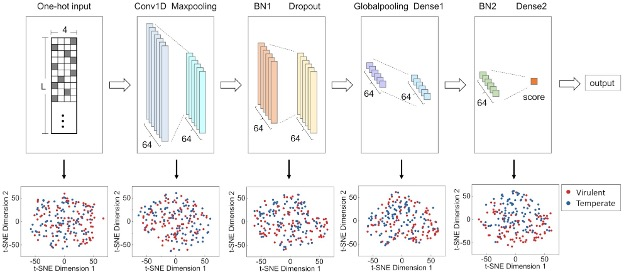
\includegraphics[width=1\linewidth]{figures/DeePhage_Model.jpg}
    \caption{Cấu trúc mạng nơ-ron học sâu và hình ảnh hóa 5 lớp bằng cách giảm kích thước của DeePhage}
    \label{fig:DeePhage_model}
\end{figure}

\subsection*{Kết quả thực nghiệm}

Dựa trên bảng kết quả kiểm thử chéo 5 lần, DeePhage vượt trộiso với PHACTS trên cả ba tiêu chí đánh giá Độ nhạy - Sensitivity, Độ đặc hiệu - Specificity và Độ chính xác- Accuracy ở tất cả các nhóm độ dài contig (từ 100–400 bp đến 1,200–1,800 bp).

Cụ thể:
\begin{itemize}
    \item Độ nhạy: DeePhage đạt từ 77.3\% đến 87.5\%, trong khi PHACTS chỉ đạt từ 64.7\% đến 73.7\%. 
    \item Độ đặc hiệu: DeePhage đạt từ 74.6\% đến 89.5\%, trong khi PHACTS chỉ đạt từ 26.3\% đến 42.3\%.
    \item Độ chính xác: DeePhage đạt độ chính xác cao từ 76.2\% đến 88.9\%, trong khi PHACTS dao động trong khoảng 48.6\% đến 54.8\%
\end{itemize}

Kết quả này cũng khẳng định ưu thế vượt trội của mô hình học sâu so với các mô hình học máy truyền thống trong việc giải quyết cùng nhiệm vụ phân loại thực khuẩn.

Ngoài ra, khi so sánh về hiệu năng, DeePhage xử lý 100 trình tự DNA chỉ mất 10s, nhanh hơn PHACTS 810 lần (135 phút)

\section{PhaTYP}

PhaTYP\cite{shang2023phatyp} là một mô hình học sâu thực hiện nhiệm vụ phân loại thực khuẩn thể trên dữ liệu metagenomics, tương tự như DeePhage. Tuy nhiên, thay vì sử dụng mạng nơ-ron tích chập (CNN) như DeePhage, PhaTYP áp dụng kiến trúc \textbf{BERT} (\textit{Bidirectional Encoder Representations from Transformers}). 

\subsection*{Chiến lược huấn luyện}

PhaTYP được huấn luyện qua hai nhiệm vụ: Học tự giám sát và Tinh chỉnh. 
\begin{itemize}
    \item \textbf{Nhiệm vụ học tự giám sát (Self-supervised learning)}: Mô hình học biểu diễn chuỗi DNA bằng cách dự đoán các đoạn bị che khuất tương tự như BERT trong xử lý ngôn ngữ tự nhiên.
    \item \textbf{Nhiệm vụ tinh chỉnh (Fine-tuning)}: Sau khi học biểu diễn DNA, mô hình được tinh chỉnh để phân loại thực khuẩn.
\end{itemize}
\begin{figure}[H]
    \centering
    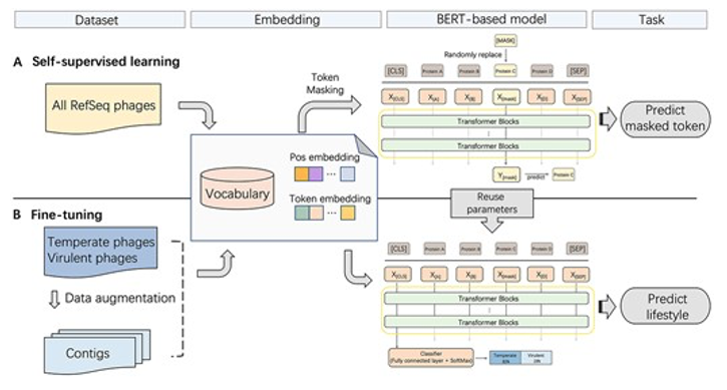
\includegraphics[width=1\linewidth]{figures/PhaTYP_Model.png}
    \caption{Kiến trúc mô hình PhaTYP sử dụng BERT}
    \label{fig:enter-label}
\end{figure}

\subsection*{Tập dữ liệu sử dụng}
\paragraph{Giai đoạn học tự giám sát:} dữ liệu được lấy từ cơ sở dữ liệu \textbf{NCBI RefSeq 2022}, bao gồm tổng cộng 3474 bộ gen của thực khuẩn. Mỗi bộ gen được cắt thành các đoạn có độ dài khác nhau: 5, 10, 15 và 20 kilobase pairs (kbp). Đối với mỗi bộ gen, 10 đoạn contig ngẫu nhiên được tạo ra, dẫn đến tổng cộng \textbf{142,434} đoạn contig được thu thập để phục vụ quá trình huấn luyện mô hình.

\paragraph{Giai đoạn phân loại:} dữ liệu được lấy từ cùng nguồn \textbf{NCBI RefSeq 2022} như ở giai đoạn học tự giám sát. Tập dữ liệu bao gồm 1290 thực khuẩn thể độc lực (\textit{virulent}) và 577 thực khuẩn thể ôn hoà (\textit{temperate}). Từ mỗi loại, 10.000 contig được tạo ngẫu nhiên với độ dài nằm trong khoảng từ 100 base pairs (bp) đến 20 kilobase pairs (kbp). Tổng cộng, tập dữ liệu huấn luyện cho giai đoạn này gồm \textbf{160,000 contig}, được xây dựng sao cho cân bằng giữa hai lớp.

\subsection*{Phương pháp và kỹ thuật chính}
PhaTYP sử dụng biểu diễn k-mer và kiến trúc BERT để học đặc trưng ngữ nghĩa của DNA, sau đó tinh chỉnh cho nhiệm vụ phân loại vòng đời thực khuẩn thể. 

Cụ thể:
\begin{itemize}
    \item Sử dụng biểu diễn DNA dưới dạng chuỗi k-mer làm đầu vào (tương tự token trong NLP).
    \item Áp dụng kiến trúc Transformer của BERT để học biểu diễn ngữ nghĩa của DNA.
    \item Tinh chỉnh lớp đầu ra cho nhiệm vụ phân loại thực khuẩn.
\end{itemize}

\subsection*{Kết quả thực nghiệm}

Dựa trên kết quả so sánh hiệu suất trên tập dữ liệu kiểm tra có mức độ tương đồng thấp, có thể nhận thấy rằng \textbf{PhaTYP vượt trội rõ rệt so với cả DeePhage và PHACTS} ở cả ba tiêu chí: độ nhạy (Sensitivity), độ đặc hiệu (Specificity) và độ chính xác (Accuracy).

\begin{table}[ht]
\centering
\caption{So sánh hiệu suất của PhaTYP với các công cụ khác.}
\label{tab:PhaTPY_Result}
\begin{tabular}{|l|c|c|c|}
\hline
\textbf{Công cụ} & \textbf{Sensitivity} & \textbf{Specificity} & \textbf{Accuracy} \\
\hline
PhaTYP             & \textbf{0.99} & \textbf{0.89} & \textbf{0.94} \\
PhaTYP (without SSL)   & 0.98 & 0.86 & 0.92 \\
DeePhage           & 0.96 & 0.86 & 0.91 \\
BACPHLIP           & 0.98 & 0.84 & 0.90 \\
PHACTS             & 0.90 & 0.69 & 0.74 \\
PhagePred          & 0.57 & 0.83 & 0.67 \\
\hline
\end{tabular}
\end{table}

So với DeePhage, PhaTYP đạt độ nhạy cao hơn (0.99 so với 0.96), độ đặc hiệu cao hơn (0.89 so với 0.86), và tổng độ chính xác cũng cao hơn (0.94 so với 0.91). Mặc dù mức chênh lệch không quá lớn, kết quả này cho thấy việc áp dụng học tự giám sát (\textit{Self-Supervised Learning – SSL}) và kiến trúc BERT đã giúp PhaTYP học được các đặc trưng ngữ nghĩa hiệu quả hơn từ dữ liệu DNA, đặc biệt trong các mẫu khó và ít tương đồng.

So với PHACTS là công cụ sử dụng mô hình học máy truyền thống, PhaTYP tạo ra kết quả khác biệt lớn. PHACTS chỉ đạt 0.90 về độ nhạy, 0.69 về độ đặc hiệu và 0.74 về độ chính xác – thấp hơn nhiều so với PhaTYP ở mọi chỉ số. 

Những điều này cho thấy khả năng vượt trội của các mô hình học sâu khi thực hiện phân loại trên dữ liệu metagenomics. Từ đó, PhaTYP khẳng định khả năng ứng dụng hiệu quả trong thực tế với nhiệm vụ phân loại thực khuẩn.

\section{DeepPL}
Tương tự PhaTYP, DeepPL\cite{zhang2024deeppl} là một mô hình phân loại vòng đời thực khuẩn thể được phát triển dựa trên kiến trúc \textbf{DNABERT} – phiên bản thích ứng của BERT cho dữ liệu chuỗi DNA. Điểm khác biệt của DeepPL là tập trung khai thác thông tin từ các đoạn gen liên quan đến chu kì tiềm tan, vốn chỉ có ở phage ôn hoà, nhằm cải thiện độ chính xác trong phân loại.

\subsection*{Dữ liệu sử dụng}

\textbf{Tập huấn luyện}:
\begin{itemize}
    \item 1262 bộ gen thực khuẩn thể độc lực
    \item 557 bộ gen thực khuẩn thể ôn hoà
\end{itemize}
    
\textbf{Tập kiểm thử}:
\begin{itemize}
    \item 245 bộ gen thực khuẩn thể độc lực
    \item 129 bộ gen thực khuẩn thể ôn hoà
\end{itemize}
    
\textbf{Tiền xử lí dữ liệu:}
Do chỉ có các thực khuẩn thể ôn hòa mới có các gen kích hoạt/duy trình chu kỳ tiềm tan, nhóm tác giả thực hiện trích xuất những đoạn gen có chức năng này. Tiếp theo, thực hiện thao tác chuẩn hoá dữ liệu:
\begin{itemize}
    \item Loại bỏ các đoạn gen nếu có nhiều hơn 10 ký tự không thuộc loại \texttt{A, T, G, C}.
    \item Với các đoạn có không quá 10 ký tự không hợp lệ, thay thế ngẫu nhiên thành A, T, G hoặc C.
\end{itemize}


\subsection*{Chiến lược tạo mẫu}
Mục tiêu của giai đoạn này, nhóm tác giả muốn tạo mẫu cân bằng giữa hai nhãn. Trong khi đặc điểm của các mẫu gen của thực khuẩn thể ôn hoà thường rất ngắn, còn mẫu gen của thực khẩn thể độc lực thường dài hơn. Do đó, nhóm tác giả dùng kĩ thuật cửa sổ trượt với kích thước cửa sổ là 100bp nhưng với các bước trượt khác nhau:
\begin{itemize}
    \item Với mẫu gen của thực khuẩn thể ôn hoà: bước trượt chỉ 1 bp để tạo ra nhiều mẫu hơn.
    \item Với mẫu gen của thực khuẩn thể ôn hoà: bước trượt 91 bp để tạo ra số mẫu tương đương.
\end{itemize}
Kết quả thu được 547{,}810 chuỗi từ gen thực khuẩn thể độc lực và 500{,}765 chuỗi từ gen thực khuẩn thể ôn hoà. Gần đạt được tỉ lệ cân bằng (50:50) đối với hai nhãn.

\subsection*{Phương pháp và kiến trúc mô hình}

\begin{itemize}
    \item \textbf{Tiền xử lý}: Chuỗi DNA được chia thành các đoạn \textit{6-mer}, tạo thành chuỗi tương tự văn bản.
    \item \textbf{Biểu diễn}: Sử dụng mô hình huấn luyện trước DNABERT để ánh xạ các 6-mer sang không gian vector.
    \item \textbf{Tinh chỉnh}: Tinh chỉnh DNABERT trên tập dữ liệu đã gán nhãn để thực hiện phân loại thực khuẩn.
\end{itemize}
\begin{figure}[H]
    \centering
    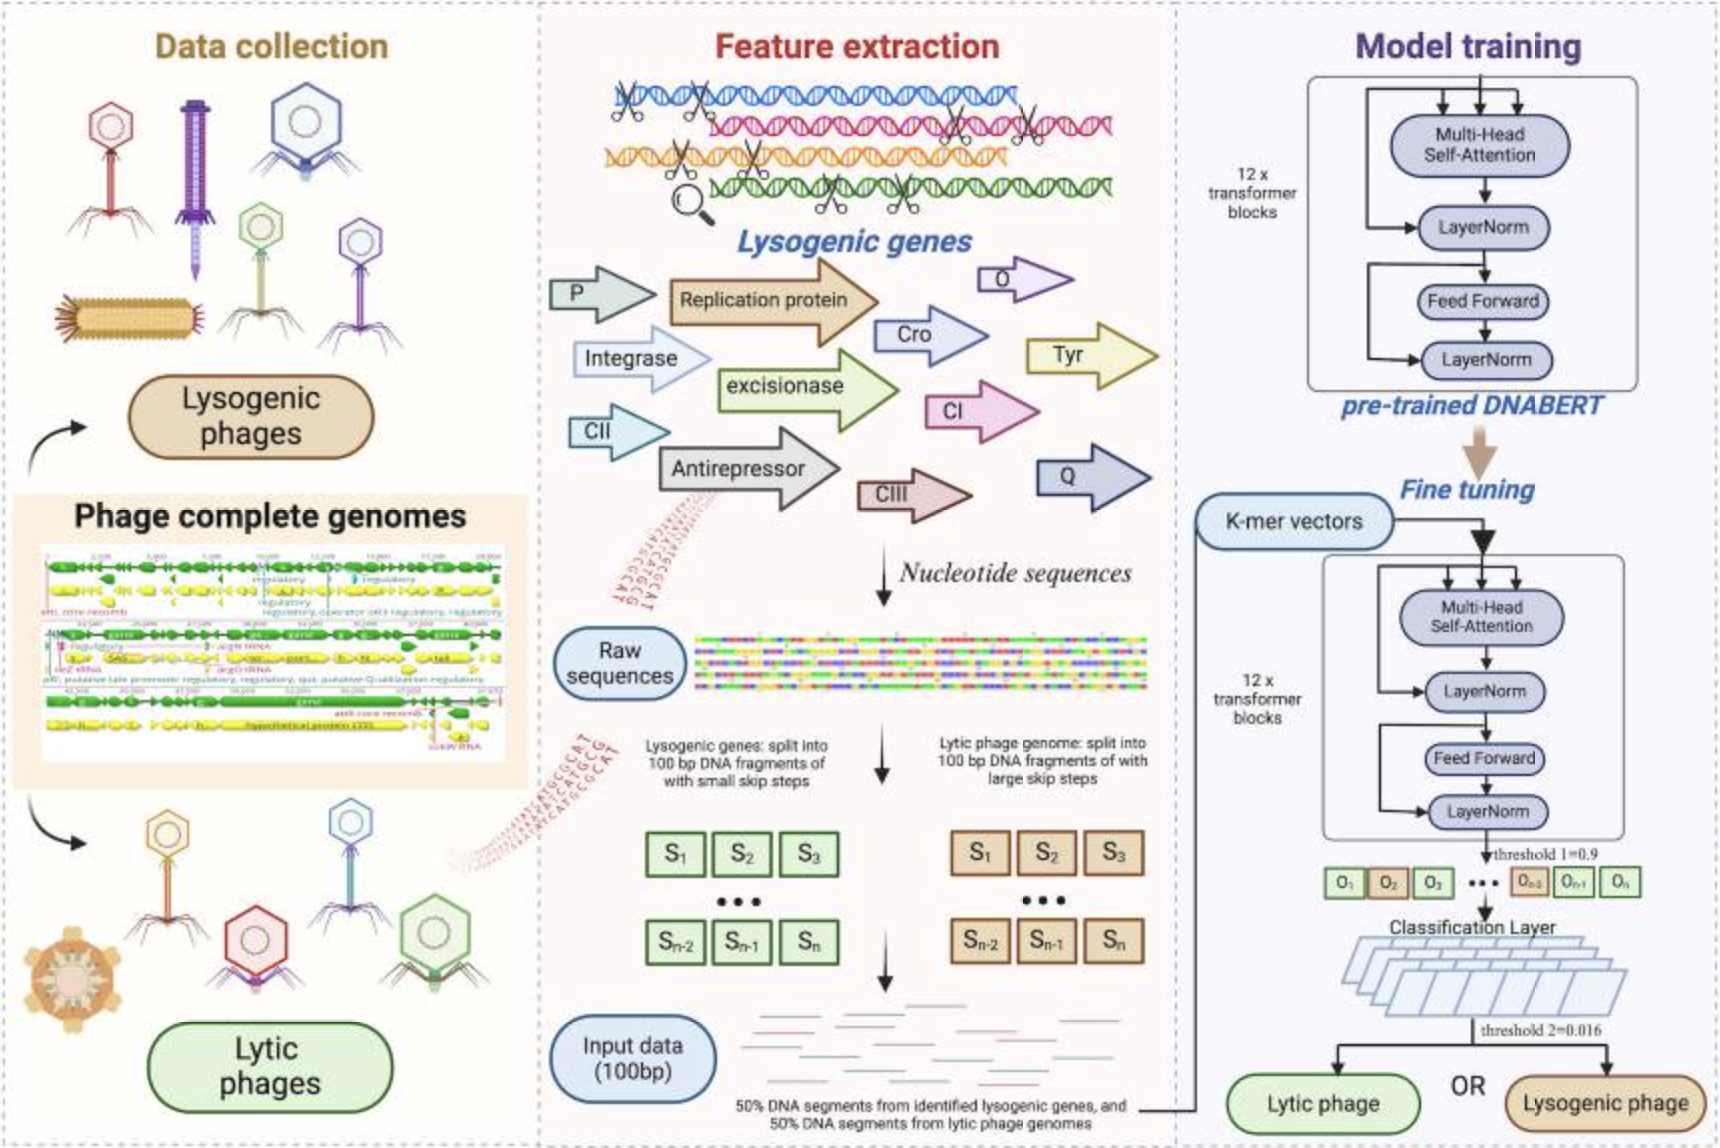
\includegraphics[width=1\linewidth]{figures/DeepPL_model.png}
    \caption{Kiến trúc mô hình DeepPL sử dụng NDABERT}
    \label{fig:DeepPL_model}
\end{figure}

\subsection*{Kết quả thực nghiệm}

\begin{table}[ht]
\centering
\caption{So sánh hiệu suất giữa DeepPL và các công cụ khác.}
\label{tab:performance_comparison_deeppl}
\begin{tabular}{|l|c|c|c|c|c|}
\hline
\textbf{Công cụ} & \textbf{Sensitivity} & \textbf{Specificity} & \textbf{Accuracy} & \textbf{F1-score} & \textbf{MCC} \\
\hline
DeepPL   & \textbf{92.24}  & 95.91 & 94.65 & 0.92 & 0.53 \\
PhaTYP   & 90.44 & 97.47 & \textbf{94.91} & 0.92 & 0.53 \\
DeePhage & 78.61 & \textbf{98.13} & 89.83 & 0.86 & 0.49 \\
PHACTS   & 38.94 & 79.77 & 48.66 & 0.53 & 0.14 \\
PhageAI  & 83.33 & 96.08 & 91.17 & 0.87 & 0.50 \\
\hline
\end{tabular}
\label{tbl:deeppl}
\end{table}

\textbf{DeepPL} cho thấy hiệu suất cao và ổn định trong bài toán phân loại thực khuẩn, với độ nhạy 92.24\%, độ đặc hiệu 95.91\%, độ chính xác 94.65\%, F-score đạt 0.92 và hệ số tương quan Matthews (MCC) là 0.53.

So với PhaTYP, DeepPL không tạo được sự khác biệt lớn. DeepPL đạt độ nhạy cao hơn (92.24\% so với 90.44\%). Nhưng so sánh độ chính xác tổng thể, DeepPL (94.65\%) thấp hơn so với PhaTYP (94.91\%).\newpage\cleardoublepage
\chapter{Thực nghiệm}
Để có cái nhìn tổng quan về các phương pháp đã đề cập đến ở chương trước, nhóm báo cáo đã tiến hành tổng hợp bộ dữ liệu được sử dụng của mỗi phương pháp và tổng hợp kết quả so sánh được đề cập trong mỗi phương pháp. Chương này trình bày bảng tổng hợp bộ dữ liệu, xây dựng bộ dữ liệu chung, sử dụng bộ dữ liệu chung để tiến hành các thực nghiệm trên 3 phương pháp là PHACTS, Phage AI và DeePhage. Cuối cùng, nhóm báo cáo sẽ trình bày kết quả thực nghiệm và phân tích kết quả.

\section{Xây dựng bộ dữ liệu}
Do các phương pháp sử dụng nhiều bộ dữ liệu khác nhau, việc so sánh trực tiếp hiệu suất phân loại giữa chúng là bất khả thi. Vì vậy, nhóm báo cáo thực hiện xây dựng một bộ dữ liệu chung để sử dụng cho các thực nghiệm của mình.
\subsection*{ Xử lý nhãn }
Bộ dữ liệu mà nhóm báo cáo xây dựng là sự kết hợp của 2 bộ được sử dụng trong bài báo DeepPL và DeePhage. Nhãn $y$ của bản ghi $X$ được nhóm báo cáo xử lý như sau:
\begin{enumerate}
    \item Nếu $X \in DeePhage \Rightarrow y = y_{DeePhage}$ 
    \item Nếu $X \in DeepPL \Rightarrow y = y_{DeepPL}$
    \item Nếu $X \in DeePhage \cap DeepPL \Rightarrow y = y_{DeePhage}$
\end{enumerate}
Sau khi kết hợp, bộ dữ liệu thu được bao gồm: 2241 bộ dữ liệu di truyền thực khuẩn, trong đó có 1534 bản ghi được gán nhãn là 1 (thực khuẩn thể độc lực) và 707 bản ghi được gán nhãn 0 (thực khuẩn thể ôn hòa). Sau đó, tập được chia nhỏ thành 2 tập: huấn luyện và kiểm thử. Trong đó, tập huấn luyện gồm 1733 bản ghi với số lượng nhãn 1 và 0 lần lượt là 1184 và 549. Tập kiểm thử có số lượng nhãn 1 và 0 lần lượt là 296 và 138.

\section{Kịch bản thực nghiệm}\label{ kịch bản thực nghiệm}
Nhóm báo cáo thực hiện mô phỏng lại 3 phương pháp: PHACTS, PhageAI và DeePhage trên bộ dữ liệu chung. Ngoài ra, nhóm có thử nghiệm phân loại bộ dữ liệu với mô hình XGBoost và so sánh mô hình này với phương pháp DeePhage.

\section{Các chỉ số đánh giá}
Để đánh giá 1 cách toàn diện hiệu suất phân loại của mô hình chứ không chỉ tập trung vào nhãn 1, nhóm báo cáo sử dụng các chỉ số sau:
\begin{itemize}
    \item Accuracy: sử dụng để do lường hiệu suất phân loại chung của mô hình trên 2 nhãn.
    \item Sensitivity: sử dụng để đo lường dộ phủ của mô hình trên nhãn 1.
    \item Specificity: sử dụng để đo lường độ phủ của mô hình trên nhãn 0.
\end{itemize}

\section{Kết quả}
\subsection{Thực nghiệm với mô hình PHACTS}
Dựa trên mã nguồn mà nhóm tác giả công bố, nhóm đã thực hiện đánh giá phương pháp PHACTS trên bộ dữ liệu của mình. Mã nguồn được công bố được thiết kế với đầu vào là dữ liệu amino axit nên nhóm cần thực hiện chuyển đổi dữ liệu di truyền sang dạng này. Để có kết quả khách quan nhất, kết quả thực nghiệm là trung bình cộng của 10 lần lặp lại.

\begin{table}[H]
    \centering
    \begin{tabular}{|m{5cm}|m{5cm}|>{\raggedleft\arraybackslash}m{3cm}|}
        \hline
        Chỉ số & Giá trị & Độ lệch chuẩn\\
        \hline
        Accuracy & 71.24\% & 1.67\%\\
        \hline
        Sensitivity & 82.77\% & 2.25\%\\
        \hline
        Specificity & 46.52\% & 3.22\%\\ 
        \hline
    \end{tabular}
    \caption{Kết quả thực nghiệm với mô hình PHACTS}
    \label{tab:result_phacts}
\end{table}

Nhóm báo cáo nhận thấy rằng, với bộ dữ liệu dùng chung ở trên, mô hình PHACTS cho kết quả Accuracy là 71.24\%, Sensitivity là 82.77\% và Specificity là 46.52\%. Kết quả này thấp hơn nhiều so với kết quả công bố của nhóm tác giả PHACTS (đã đề cập ở phần trước).

\subsection{Kết quả thực nghiệm với PhageAI}
Nhóm báo cáo thực hiện thử nghiệm các thuật toán học máy trong bài báo PhageAI với bộ dữ liệu mới. Các mô hình đều sử dụng BayesianSearch để tối ưu lựa chọn các bộ tham số tốt nhất. Riêng với thuật toán SVM, nhóm báo cáo sử dụng bộ tham số đã được tác giả công bố trong bài báo.
\begin{table}[ht]
\footnotesize
\centering
\begin{tabular}{|l|c|c|c|}
\hline
\textbf{Model} & \textbf{Accuracy} & \textbf{Sensitivity (Class 1)} & \textbf{Specificity (Class 0)} \\
\hline
GaussianNB & 0.649 & 0.780 & 0.365 \\
SGDClassifier & 0.864 & 0.861 & 0.869 \\
MLPClassifier & 0.901 & 0.946 & 0.803 \\
RandomForestClassifier & 0.928 & \textbf{0.963} & 0.854 \\
SVC & 0.901 & 0.882 & \textbf{0.942} \\
KNeighborsClassifier & 0.910 & 0.909 & 0.912 \\
GradientBoostingClassifier & 0.930 & 0.951 & 0.882 \\
XGBoost & \textbf{0.936} & 0.959 & 0.883 \\
LightGBM & 0.933 & 0.951 & 0.878 \\
CatBoost & 0.931 & 0.953 & 0.870 \\
\hline
\end{tabular}


\caption{Kết quả so sánh các thuật toán học máy theo Accuracy, Sensitivity và Specificity trên bộ dữ liệu kết hợp.}
\label{tab:model_comparison}
\end{table}

Dựa trên kết quả Bảng \ref{tab:model_comparison}, có thể thấy rằng các mô hình thuộc nhóm ensemble learning, đặc biệt là các thuật toán Boosting như XGBoost, LightGBM, CatBoost và GradientBoostingClassifier, đều cho hiệu suất rất cao trên cả ba chỉ số: Accuracy, Sensitivity và Specificity. Trong đó, XGBoost đạt Accuracy cao nhất (0.936), đồng thời duy trì mức Sensitivity (0.959) và Specificity (0.883) rất cân bằng, cho thấy khả năng phân biệt tốt giữa hai lớp.

RandomForestClassifier cũng thể hiện hiệu quả cao với Accuracy 0.928, tuy nhiên có phần thiên lệch hơn về Sensitivity (0.963) so với Specificity (0.854), nghĩa là mô hình có xu hướng nhạy hơn với lớp dương (Class 1). Khi so sánh kết quả này với PHACTS cũng sử dụng RandomForestClassifier, có thể thấy rằng PHACTS có độ chính xác thấp hơn nhiều (71.24\%) và độ nhạy cũng thấp hơn (82.77\%) so với các mô hình học máy hiện đại. 

Ở nhóm mô hình cơ bản hơn như GaussianNB và SGDClassifier, kết quả không thực sự khả quan. Đặc biệt, GaussianNB cho Specificity chỉ ở mức 0.365, cho thấy mô hình này khó phân biệt được lớp âm (Class 0), mặc dù có Sensitivity tương đối tốt (0.780). Điều này thường xảy ra khi dữ liệu không phù hợp với giả định phân phối chuẩn của Naive Bayes.

MLPClassifier và SVC đều có Accuracy trên 0.9, nhưng mỗi mô hình có thiên hướng riêng: MLPClassifier nghiêng về phát hiện Class 1 (Sensitivity cao 0.946), trong khi SVC lại rất mạnh trong việc nhận diện Class 0 (Specificity 0.942).

Tổng thể, như vậy khác với tập dữ liệu của bài báo với SVC cho kết quả tốt nhất thì trong thực nghiệm này, các mô hình Boosting như XGBoost và GradientBoostingClassifier tỏ ra vượt trội về độ chính xác và cân bằng giữa các chỉ số, phù hợp với các bài toán phân loại nhị phân có yêu cầu cao về độ tin cậy. 

\subsection{So sánh hiệu suất phân loại giữa DeePhage và XGBoost trên bộ dữ liệu xây dựng}

\begin{figure}[H]
    \centering
    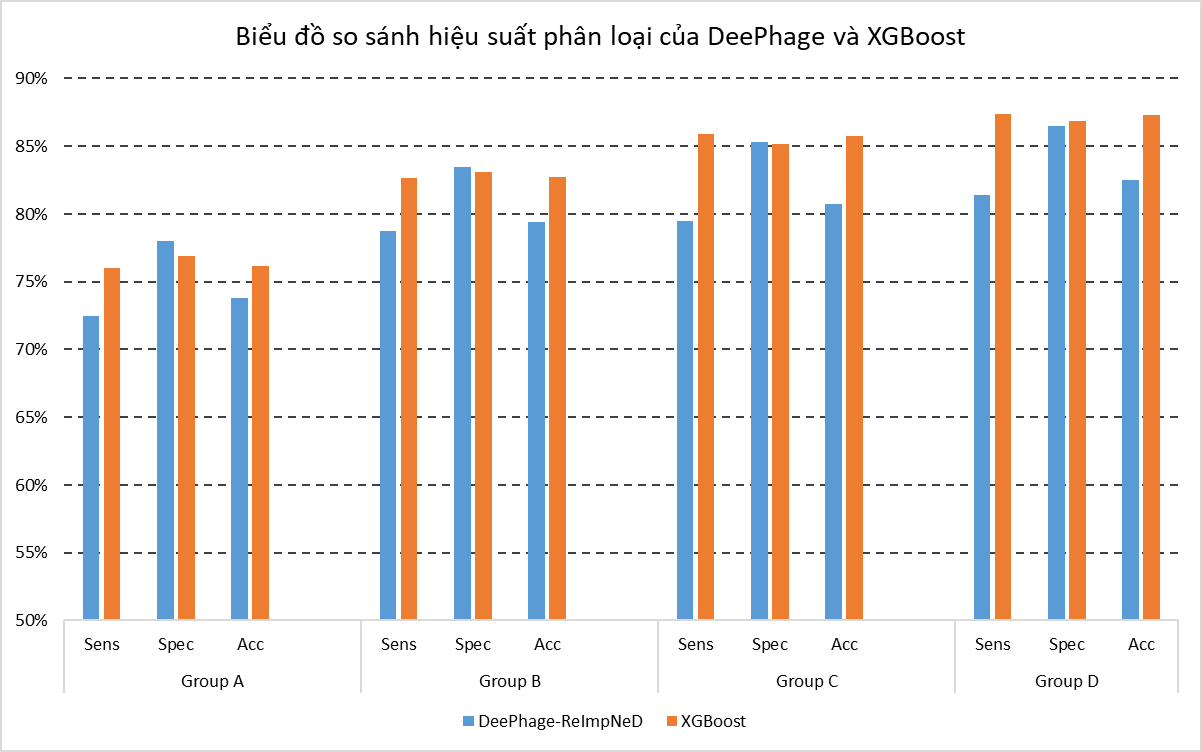
\includegraphics[width=1\linewidth]{figures/result_deephage_vs_xgboost.png}
    \caption{Kết quả hiệu suất phân loại của mô hình XGBoost trên tập dữ liệu xây dựng.}
    \label{fig:result_2}
\end{figure}

Hình \ref{fig:result_2} là biểu đồ so sánh hiệu suất phân loại của DeePhage và XGBoost trên tập dữ liệu mà nhóm báo cáo xây dựng. Có thể thấy, DeePhage cho kết quả tốt hơn 1 chút, khoảng từ 2\% - 5\% khi hơn XGBoost ở 2 chỉ số Sensitivity và Accuracy. Nghĩa là DeePhage cho khả năng nhận diện nhãn 1 và độ chính xác tổng thể cao hơn. Với chỉ số Specificity, XGBoost cho kết quả tốt hơn khoảng 5\%, nghĩa là khả năng nhận diễn nhãn 0 của XGBoost tốt hơn DeePhage.

\newpage\cleardoublepage

\chapter{Kết luận}
\section{Thảo luận mở rộng}

\subsection{Vấn đề về tính giải thích của mô hình}

Một trong những thách thức lớn nhất hiện nay trong việc áp dụng các mô hình học sâu vào phân loại thực khuẩn thể là tính khó giải thích (\textit{interpretability}). Các mô hình như \textbf{DeepPL} hay \textbf{PhaTYP} hoạt động như “hộp đen”, khiến cho việc truy vết nguyên nhân sinh học đằng sau dự đoán trở nên khó khăn.

\begin{itemize}
    \item Với các mô hình truyền thống như \textbf{PHACTS} hay \textbf{BACPHLIP}, các đặc trưng (như protein domain, mức độ tương đồng protein) dễ dàng liên hệ với kiến thức sinh học.
    \item Trong khi đó, các mô hình học sâu chỉ cung cấp đầu ra phân loại mà không lý giải cụ thể đặc trưng nào ảnh hưởng tới kết quả.
\end{itemize}

Điều này gây khó khăn khi kết hợp kết quả mô hình với thực nghiệm sinh học hoặc khi cần kiểm chứng trong môi trường lâm sàng. Vì vậy, hướng nghiên cứu cần tập trung phát triển các mô hình \textbf{có khả năng giải thích} (\textit{explainable AI – XAI}) hoặc kết hợp giữa các lớp học máy và sinh học chức năng.

\subsection{Khả năng mở rộng và cập nhật mô hình}

Hầu hết các mô hình hiện nay đều cần \textbf{tái huấn luyện khi có dữ liệu mới}, đặc biệt là các mô hình học sâu như PhageAI hay DeepPL. Điều này gây khó khăn trong thực tiễn vì:

\begin{itemize}
    \item Dữ liệu thực khuẩn thể liên tục được cập nhật.
    \item Tập huấn luyện cần duy trì độ cân bằng giữa hai vòng đời.
    \item Yêu cầu phần cứng lớn khi huấn luyện lại mô hình với toàn bộ dữ liệu.
\end{itemize}

Do đó, hướng tiếp cận \textbf{học liên tục} (\textit{continual learning}) hoặc \textbf{học bán giám sát} (\textit{semi-supervised learning}) có thể là giải pháp tiềm năng, cho phép mô hình thích ứng dần với dữ liệu mới mà không cần tái huấn luyện hoàn toàn.

\subsection{Ứng dụng trong môi trường metagenomics}

Dữ liệu metagenomics là môi trường đặc biệt, chứa nhiều contig ngắn chưa rõ nguồn gốc. Các phương pháp như \textbf{DeePhage} và \textbf{PhaTYP} cho thấy khả năng vượt trội trong việc xử lý loại dữ liệu này, tuy nhiên vẫn tồn tại các giới hạn:

\begin{itemize}
    \item Các contig quá ngắn (<100 bp) hoặc chứa nhiều tạp nhiễu vẫn gây khó khăn cho mô hình.
    \item Thiếu annotation khiến việc xác nhận vòng đời phage ngoài thực nghiệm là bất khả thi.
\end{itemize}

Giải pháp có thể là kết hợp phân loại phage với các phương pháp xác định vị trí chèn gen, tìm gene dấu hiệu lysogeny, hoặc kết hợp thêm thông tin từ vật chủ vi khuẩn để tăng độ tin cậy.

\subsection{Kết hợp nhiều phương pháp (ensemble)}

Một hướng đi nhiều tiềm năng là xây dựng hệ thống phân loại phage đa tầng (multi-stage pipeline), kết hợp nhiều mô hình:

\begin{itemize}
    \item Giai đoạn đầu: Lọc nhanh các contig nghi ngờ bằng DeePhage hoặc mô hình CNN đơn giản.
    \item Giai đoạn hai: Áp dụng DeepPL hoặc DNABERT để phân tích chuyên sâu.
    \item Giai đoạn ba: Ánh xạ kết quả với dữ liệu protein, domain để tăng tính giải thích.
\end{itemize}

Cách tiếp cận này giúp tận dụng sức mạnh của từng mô hình, đồng thời cân bằng giữa tốc độ, độ chính xác và khả năng giải thích kết quả.

\subsection{Hướng nghiên cứu tương lai}

Dựa trên những quan sát và đánh giá ở trên, các hướng nghiên cứu tiềm năng bao gồm:

\begin{itemize}
    \item Phát triển các mô hình học sâu có khả năng giải thích (\textit{interpretable deep learning}).
    \item Ứng dụng kỹ thuật học liên tục hoặc học bán giám sát để cập nhật mô hình với chi phí thấp.
    \item Kết hợp thêm thông tin từ hệ gen vật chủ hoặc môi trường sinh học xung quanh.
    \item Chuẩn hóa tập dữ liệu benchmark để dễ dàng đánh giá mô hình một cách khách quan.
\end{itemize}\newpage\cleardoublepage
% \chapter*{Kết luận}
\addcontentsline{toc}{chapter}{Kết luận}

Tổng kết đóng góp của khảo sát...

Gợi ý hướng phát triển nghiên cứu tiếp theo...
\newpage\cleardoublepage


%\nocite{*}
\phantomsection 
\addcontentsline{toc}{chapter}{Tài liệu tham khảo}
\bibliography{references}\newpage\cleardoublepage
\bibliographystyle{plain}
\end{document}
